\section*{Introduction}

This report explains the implementation details of CS523 Computer Vision
Assignment 3, which is about classifying a 4-class dataset with bag of features.
The general idea behind a bag of visual words is to represent an image as a set
of features. Features consist of keypoints and descriptors and no matter if an
image is rotated, shrinked or expanded, the keypoints will always be the same. A
descriptor is the description of a keypoint. The keypoints and descriptors are
used to construct vocabularies and represent each image as a frequency histogram
of features that are in the image. By using the frequency histogram, we can
find and predict the category of an image.

\section*{Running the code}
To run the code, you need to re-organize the dataset to look something similar
to:

\dirtree{%
    .1 dataset.
    .2 train.
    .3 airplanes.
    .3 cars.
    .3 faces.
    .3 motorbikes.
    .2 test.
    .3 airplanes.
    .3 cars.
    .3 faces.
    .3 motorbikes.
}

After modifying the directory structure, you should call main.py with the
parameters that are needed to run the experiment you want. For example, the
following snippet will set the feature extraction method to keypoints, will use
kmeans, k=50 for the clustering algorithm.


\begin{lstlisting}[language=Bash,title=Running the code,captionpos=b]
python main.py --train_path dataset-modified/train --test_path
dataset-modified/test --no_clusters 50 --clustering_alg kmeans
--feature_extraction kp

\end{lstlisting}


\section*{Feature Extraction and Description}

Scale invariant feature transform(SIFT) is a feature detection algorithm, to detect
and describe local features in images. In order to apply SIFT, I first extracted
the features of the train images using two different methods. I first detected
keypoints in each image using sift.detectAndCompute and than constructed a
keypoint array with iterating over the image using two different step sizes, 15
and 10. For the grids, I used sift.compute.


\begin{figure}[H]
    \centering
    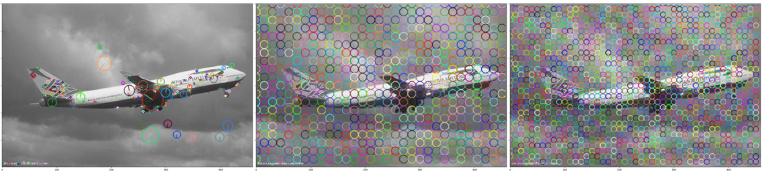
\includegraphics[width=\textwidth]{images/ext-desc.png}
    \caption*{SIFT with keypoints, grid with step\_size = 15, grid with step\_size = 10}
    \setlength{\belowcaptionskip}{-20pt}
    \setlength{\abovecaptionskip}{-20pt}
\end{figure}


\section*{Dictionary Computation, Feature quantization and Histogram Calculation}

After I got my descriptors, I vertically stacked all of them into an array and
send the vertically stacked descriptors to my clustering algorithm. After I got
my cluster, I created a histogram and ended up with the following vocablulary,
for each experiment.

\subsection*{keypoints, k-means: k = 50}
\begin{figure}[H]
    \centering
    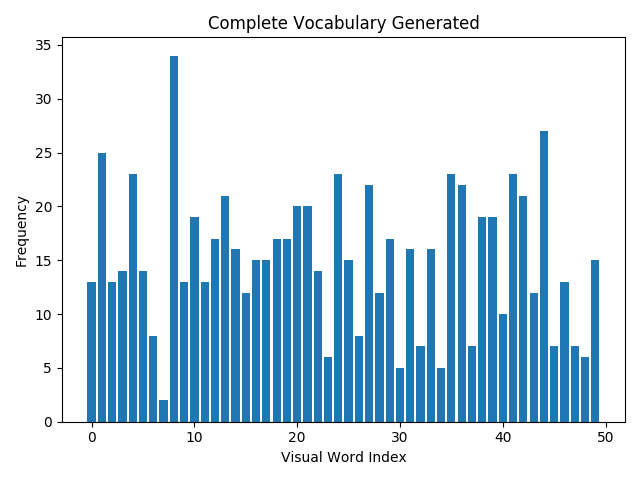
\includegraphics[width=\textwidth]{images/bow-kp-50.png}
\end{figure}

\subsection*{keypoints, k-means: k = 250}
\begin{figure}[H]
    \centering
    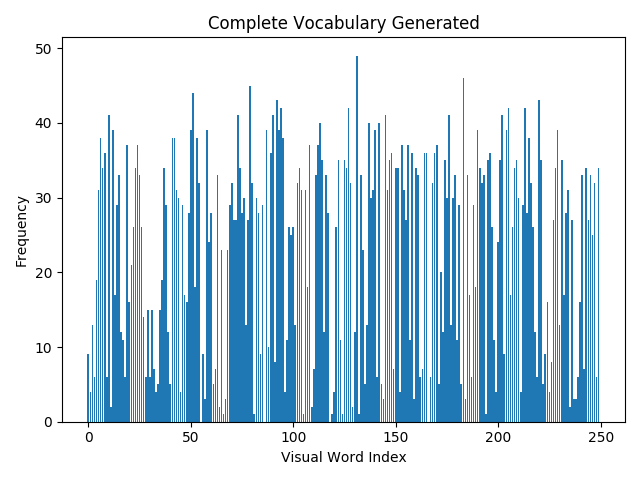
\includegraphics[width=\textwidth]{images/bow-kp-250.png}
\end{figure}

\subsection*{keypoints, k-means: k = 500}
\begin{figure}[H]
    \centering
    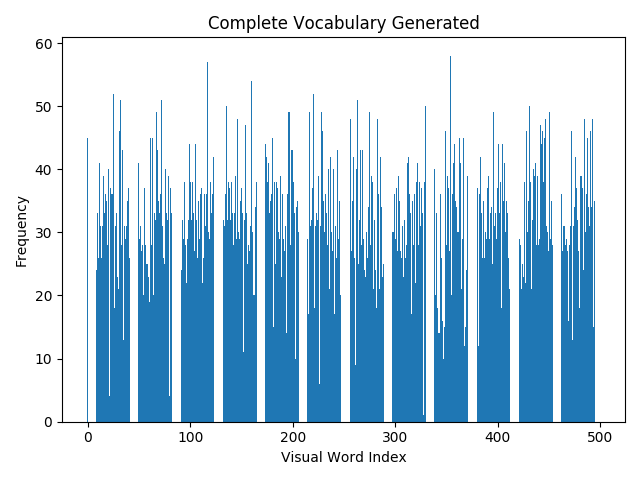
\includegraphics[width=\textwidth]{images/bow-kp-500.png}
\end{figure}

\subsection*{keypoints, k found by Mean Shift}
\subsection*{keypoints, k-means: Meanshift found k}

\subsection*{grid-1(step\_size=15), k-means: k = 50}
\begin{figure}[H]
    \centering
    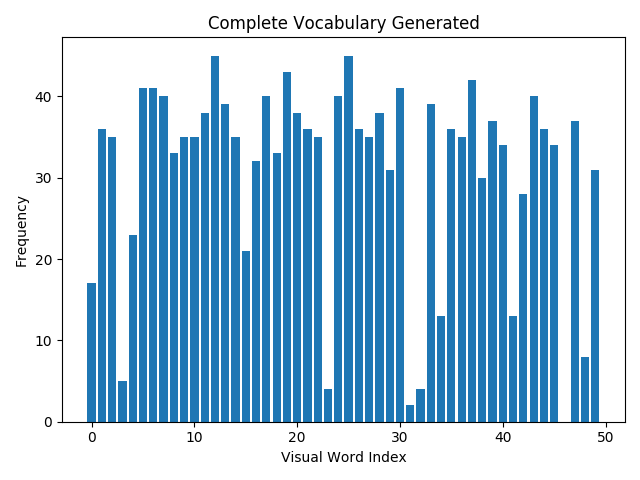
\includegraphics[width=\textwidth]{images/bow-stp-15-50.png}
\end{figure}

\subsection*{grid-1(step\_size=15), k-means: k = 250}
\begin{figure}[H]
    \centering
    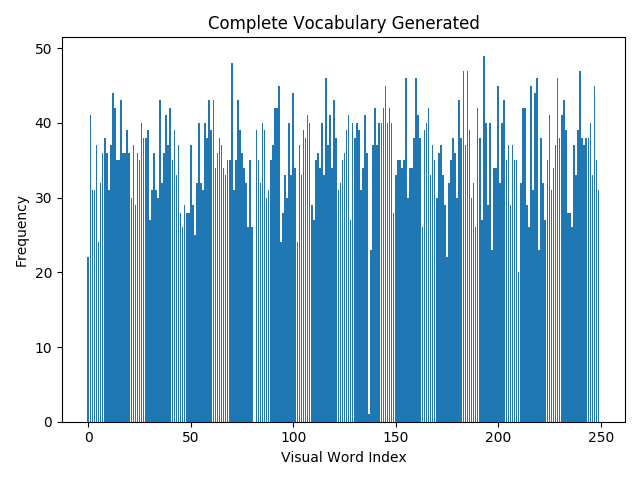
\includegraphics[width=\textwidth]{images/bow-stp-15-250.png}
\end{figure}

\subsection*{grid-1(step\_size=15), k-means: k = 500}
\begin{figure}[H]
    \centering
    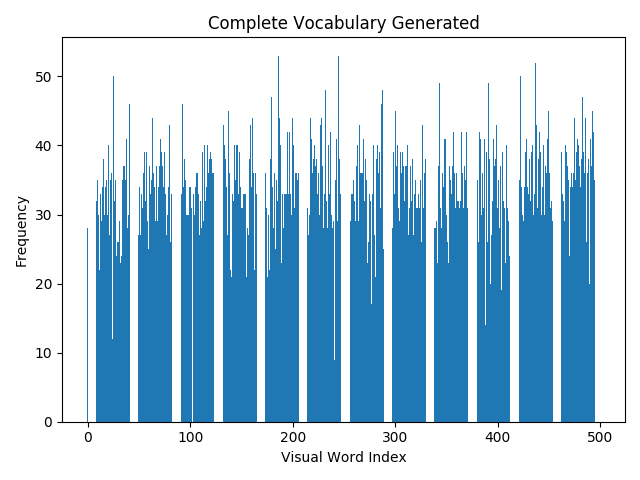
\includegraphics[width=\textwidth]{images/bow-stp-15-500.png}
\end{figure}

\subsection*{grid-1(step\_size=15), k found by Mean Shift}
\subsection*{grid-1(step\_size=15), k-means: Meanshift found k}

\subsection*{grid-2(step\_size=10), k-means: k = 50}
\begin{figure}[H]
    \centering
    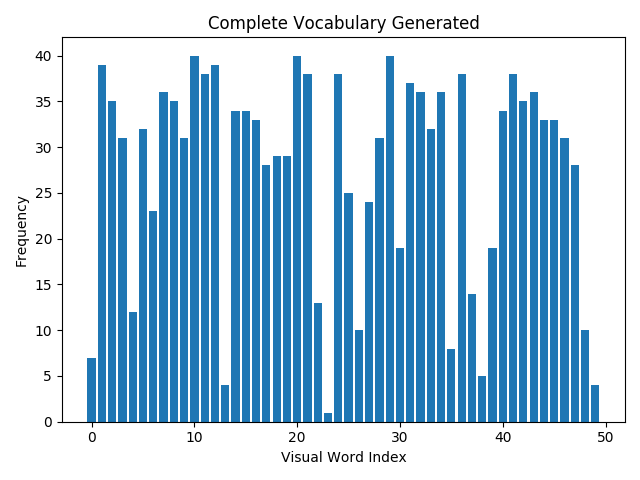
\includegraphics[width=\textwidth]{images/bow-stp-10-50.png}
\end{figure}

\subsection*{grid-2(step\_size=10), k-means: k = 250}
\begin{figure}[H]
    \centering
    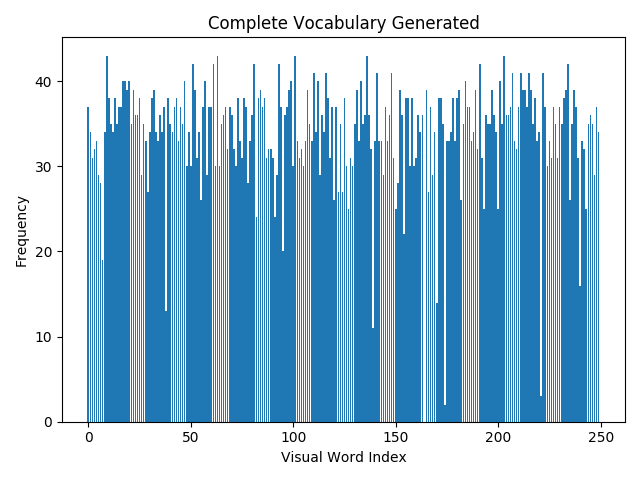
\includegraphics[width=\textwidth]{images/bow-stp-10-250.png}
\end{figure}

\subsection*{grid-2(step\_size=10), k-means: k = 500}
\begin{figure}[H]
    \centering
    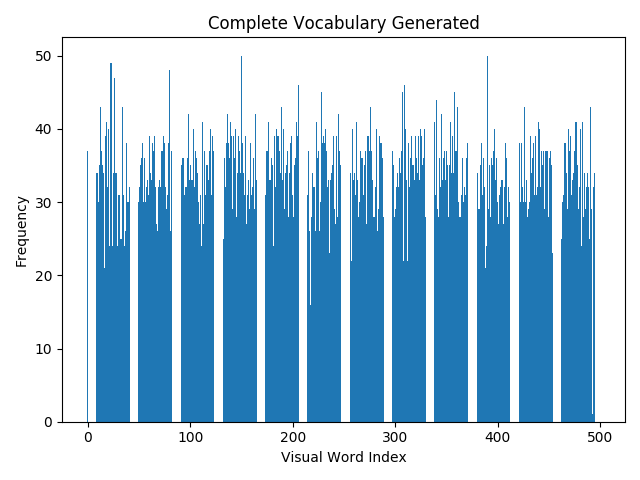
\includegraphics[width=\textwidth]{images/bow-stp-10-500.png}
\end{figure}

\subsection*{grid-2(step\_size=10), k found by Mean Shift}
\subsection*{grid-2(step\_size=10), k-means: Meanshift found k}


%\section*{Classifier Training}

\section*{Results}

\subsection*{keypoints, k-means: k = 50}
\begin{figure}[H]
    \centering
    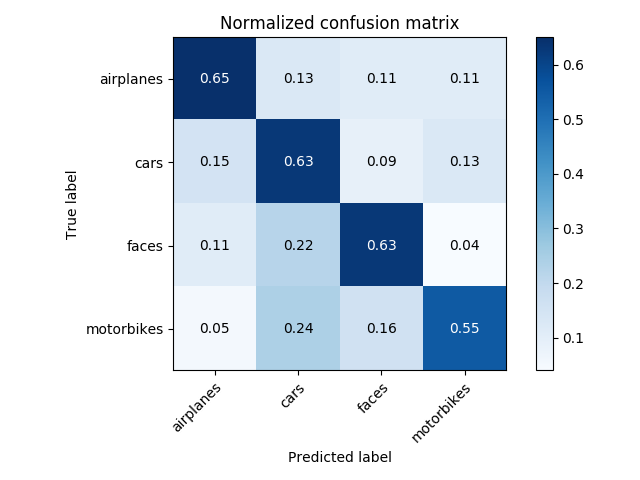
\includegraphics[width=\textwidth]{images/confusion-kp-50.png}
    \caption*{Accuracy: \%66}
\end{figure}

\subsection*{keypoints, k-means: k = 250}
\begin{figure}[H]
    \centering
    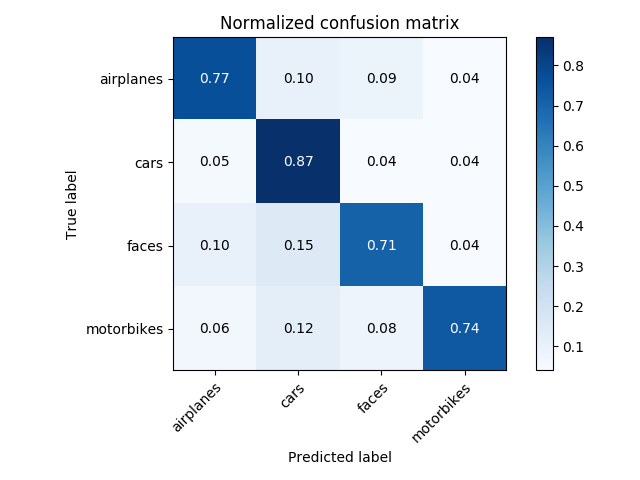
\includegraphics[width=\textwidth]{images/confusion-kp-250.png}
    \caption*{Accuracy: \%77.7}
\end{figure}

\subsection*{keypoints, k-means: k = 500}
\begin{figure}[H]
    \centering
    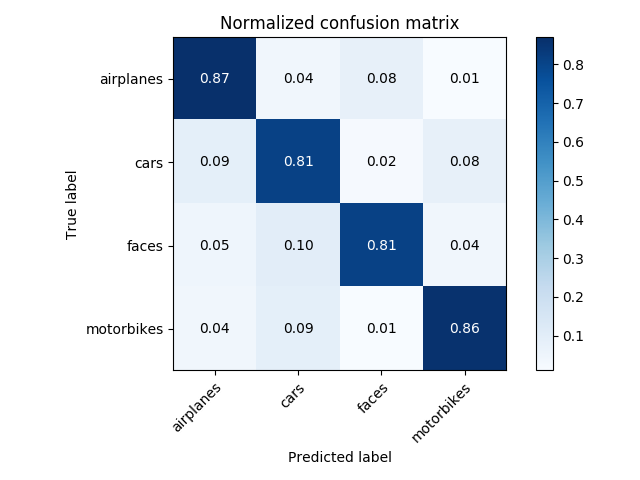
\includegraphics[width=\textwidth]{images/confusion-kp-500.png}
    \caption*{Accuracy: \%83.8}
\end{figure}

\subsection*{keypoints, k found by Mean Shift}
\subsection*{keypoints, k-means: Meanshift found k}

\subsection*{grid-1(step\_size=15), k-means: k = 50}
\begin{figure}[H]
    \centering
    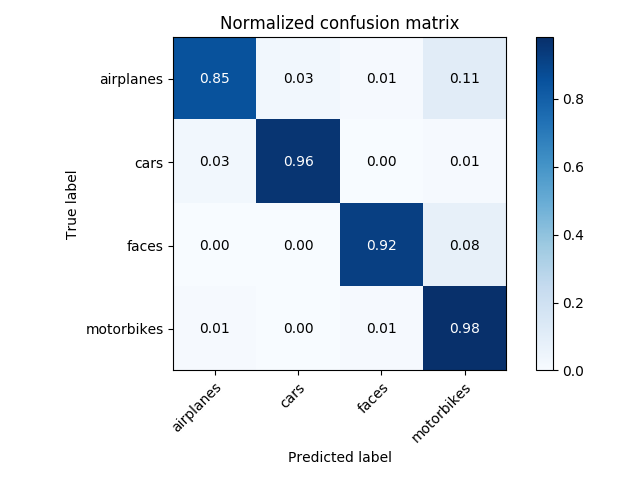
\includegraphics[width=\textwidth]{images/confusion-stp-15-50.png}
    \caption*{Accuracy: \%92.7}
\end{figure}

\subsection*{grid-1(step\_size=15), k-means: k = 250}
\begin{figure}[H]
    \centering
    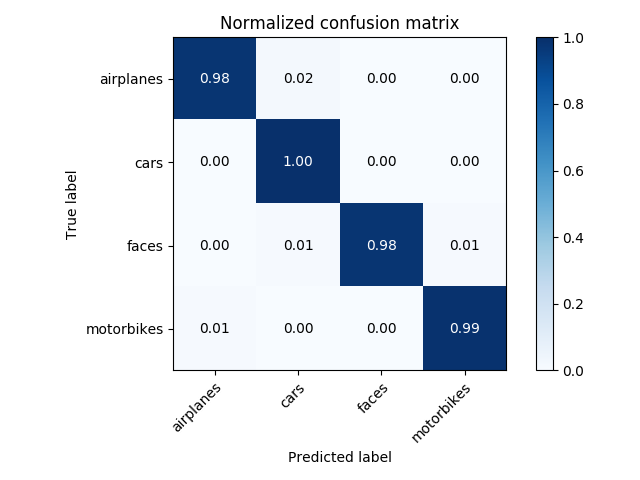
\includegraphics[width=\textwidth]{images/confusion-stp-15-250.png}
    \caption*{Accuracy: \%99}
\end{figure}

\subsection*{grid-1(step\_size=15), k-means: k = 500}
\begin{figure}[H]
    \centering
    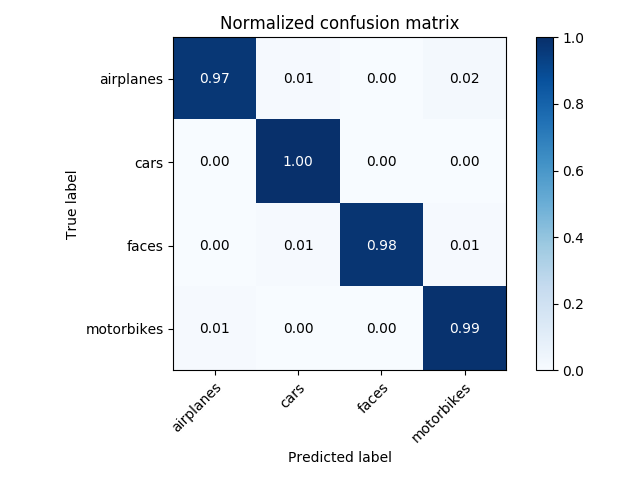
\includegraphics[width=\textwidth]{images/confusion-stp-15-500.png}
    \caption*{Accuracy: \%98.5}
\end{figure}

\subsection*{grid-1(step\_size=15), k found by Mean Shift}
\subsection*{grid-1(step\_size=15), k-means: Meanshift found k}

\subsection*{grid-2(step\_size=10), k-means: k = 50}
\begin{figure}[H]
    \centering
    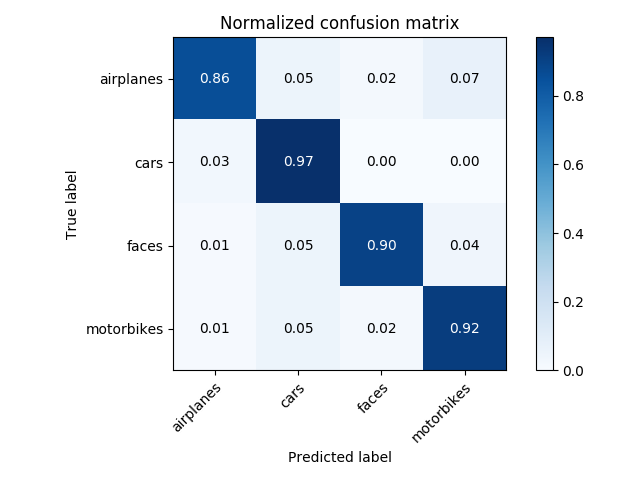
\includegraphics[width=\textwidth]{images/confusion-stp-10-50.png}
    \caption*{Accuracy: \%91.2}
\end{figure}

\subsection*{grid-2(step\_size=10), k-means: k = 250}
\begin{figure}[H]
    \centering
    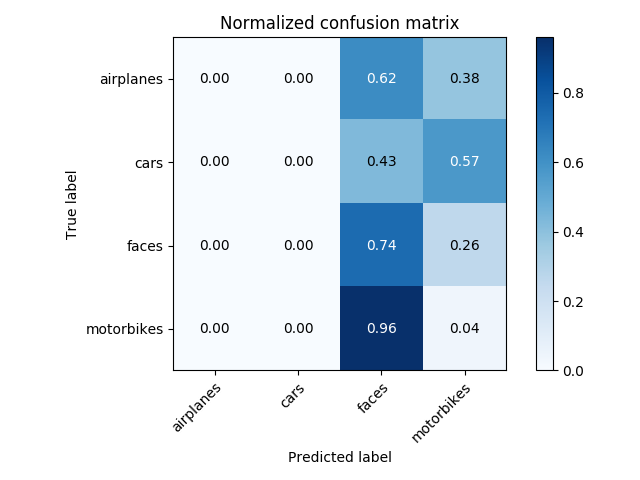
\includegraphics[width=\textwidth]{images/confusion-stp-10-250.png}
    \caption*{Accuracy: \%98.5}
\end{figure}

\subsection*{grid-2(step\_size=10), k-means: k = 500}
\begin{figure}[H]
    \centering
    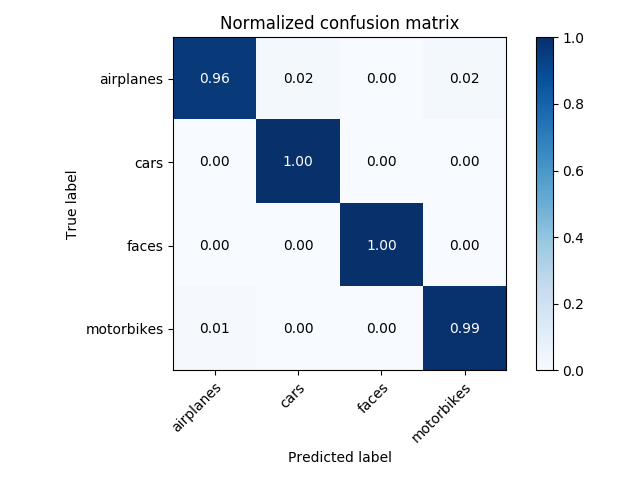
\includegraphics[width=\textwidth]{images/confusion-stp-10-500.png}
    \caption*{Accuracy: \%98.8}
\end{figure}

\subsection*{grid-2(step\_size=10), k found by Mean Shift}
\subsection*{grid-2(step\_size=10), k-means: Meanshift found k}

\section*{Comments}

